\documentclass[11pt,a4paper]{jsarticle}
%
\usepackage{amsmath,amssymb}
\usepackage{bm}
\usepackage[dvipdfmx]{graphicx}
\usepackage{ascmac}
\usepackage{url}
\usepackage{color}
\usepackage{listings}
\usepackage{booktabs}

%
\usepackage{titlesec}     % For \titleformat
\usepackage{enumerate}  % For enumerate
% \usepackage{ulem}       % For underlining
%
\titleformat*{\section}{\large\bfseries}
\titleformat*{\subsection}{\normalsize\bfseries}
%\setcounter{section}{-1}
%
\setlength{\textwidth}{\fullwidth}
\setlength{\textheight}{37\baselineskip}
\addtolength{\textheight}{\topskip}
\setlength{\voffset}{-0.5in}
\setlength{\headsep}{0.3in}
%
%\newcommand{\divergence}{\mathrm{div}\,}  %ダイバージェンス
%\newcommand{\grad}{\mathrm{grad}\,}  %グラディエント
%\newcommand{\rot}{\mathrm{rot}\,}  %ローテーション
%
\pagestyle{myheadings}
\markright{知能機械制御学研究室:\TeX 講習会の資料(当日用)}
\begin{document}

\begin{center}
  {\Large\bfseries \TeX 講習会の資料(当日用)} % title
\end{center}
\begin{flushright}
  {\large 諏訪 棟植} % author
\end{flushright}
%
%
\section{間違いのあった点}

細かい数式の違いや空白文字の有無までは指摘していません.

\subsection{文中の数式}

\verb|$$|でくくってください.(多分凡ミス)

\begin{quotation}
  f(x)のフーリエ級数展開
\end{quotation}

\subsection{インデント}

数式と文は行を開けないでください.どうしても開けたい場合は\verb|%|で埋めてください.もし,不適切な箇所で何らかの理由でインデントが行われる場合は,\verb|\noindent|を使ってください.

\begin{quotation}
  図1のように, 点Oに作用している3力$F_1,F_2,F_3$が釣り合っている時とき,
  \begin{align*}
    \frac{F_1}{\sin(\pi-\theta_1)}=\frac{F_2}{\sin(\pi-\theta_2)}=\frac{F_3}{\sin(\pi-\theta_3)} \\
  \end{align*}

  となる.
\end{quotation}

\subsection{$\sin$ vs. $sin$}

$\sin,\lim$などは,\verb|\|をつけて\verb|\sin,\lim|と書いてください.

\begin{quotation}
  \begin{align*}
    f(0^+)=lim_{t \to 0}f(t)
  \end{align*}
\end{quotation}

\subsection{式番号とか}\label{sec:equation-number}

式番号を記述する際は,\verb|\eqref{}|を利用してください.式の順序が変わったときに連動して変換されます.図や表などの\verb|\ref{}|も同様です.この例を\eqref{a}と\eqref{b}で示します.
\begin{align}
  a=1\label{a} \\
  b=1\label{b}
\end{align}
\verb#\verb|(1)|#を用いているものがありましたが,\verb|\eqref{}|とすれば,自動で数字とかっこが出力されます.

なお,\verb|\ref{}|は,\verb|\section{}|などに対しても使えます.例:\ref{sec:equation-number}節

\subsection{$\sim$ vs. ~}

日本語の波線~でなく,\verb|\sim|を使ってください.

\begin{quotation}
  $f(x)$ のフーリエ級数展開を(1)に示す.
  \begin{align}
    f(x)  〜  \frac{a_0}{2} + \sum_{n=1}^{∞} (a_n\cos\omega_n x + b_n\sin\omega_n x)
  \end{align}
\end{quotation}

\subsection{$\frac{n!}{(s+a)^{n+1}}$ vs. $n!/(s+a)^{n+1}$}

斜めの分数を書くときは\verb|/|を用いてください.

\subsection{上付き文字}

\verb|(-1)^{i+j}|などと,\verb|{}|でくくってください.(多分凡ミス)

\begin{quotation}
  余因子行列$\tilde{A}$は,余因子$A_{ij}:=(-1)^(i+j)\Delta{ij}$を用いると,
\end{quotation}

\subsection{$\hat{A}$ vs. $\tilde{A}$}

凡ミスかな?

\begin{quotation}
  余因子行列$\hat{A}$は,\quad 余因子$A_{ij}:=(-1)^{i+j}\Delta_{ij}$ を用いると,
\end{quotation}

\section{その他}

\subsection{式番号}

\verb|\begin{align*}~\end{align*}|や\verb|\nonumber|などで適宜削除してください.

\subsection{図の数式}

数式機能を使ってください.ラミの定理の図でなく,図\ref{fig:example-image}が用いられているものや図がないものがありましたが,パワポなどでPC上で作図する方法は確認しておいてください.

\begin{figure}[hbtp]
  % []の中身について,t,b,p,hはそれぞれページ上端,ページ下端,単独ページ,できればその位置に図を出力するように指定する.
  % []内の順番は優先順位を示す.
  \centering % 中央揃えを行う
  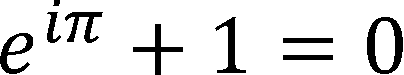
\includegraphics[width=6cm]{example-crop.pdf} % 幅の長さとファイル名を指定する.
  \caption{図の例} % 図の下にキャプションをつける
  \label{fig:example-image} % ラベルを付け,文中から図\ref{}で図"番号"とする.
\end{figure}

\subsection{図の挿入位置}

言及し忘れたかもしれませんが,図を挿入する際は,TeXファイル上にて段落の間に\verb|\begin{figure}~\end{figure}|などを記述してください.

\subsection{$\bigtriangleup$ vs. $\Delta$}

\verb|\bigtriangleup|と\verb|\Delta|のどっちが正しいかは分かりませんが,出題時は後者を使いました.

\end{document}
